\documentclass[1p]{elsarticle_modified}
%\bibliographystyle{elsarticle-num}

%\usepackage[colorlinks]{hyperref}
%\usepackage{abbrmath_seonhwa} %\Abb, \Ascr, \Acal ,\Abf, \Afrak
\usepackage{amsfonts}
\usepackage{amssymb}
\usepackage{amsmath}
\usepackage{amsthm}
\usepackage{scalefnt}
\usepackage{amsbsy}
\usepackage{kotex}
\usepackage{caption}
\usepackage{subfig}
\usepackage{color}
\usepackage{graphicx}
\usepackage{xcolor} %% white, black, red, green, blue, cyan, magenta, yellow
\usepackage{float}
\usepackage{setspace}
\usepackage{hyperref}

\usepackage{tikz}
\usetikzlibrary{arrows}

\usepackage{multirow}
\usepackage{array} % fixed length table
\usepackage{hhline}

%%%%%%%%%%%%%%%%%%%%%
\makeatletter
\renewcommand*\env@matrix[1][\arraystretch]{%
	\edef\arraystretch{#1}%
	\hskip -\arraycolsep
	\let\@ifnextchar\new@ifnextchar
	\array{*\c@MaxMatrixCols c}}
\makeatother %https://tex.stackexchange.com/questions/14071/how-can-i-increase-the-line-spacing-in-a-matrix
%%%%%%%%%%%%%%%

\usepackage[normalem]{ulem}

\newcommand{\msout}[1]{\ifmmode\text{\sout{\ensuremath{#1}}}\else\sout{#1}\fi}
%SOURCE: \msout is \stkout macro in https://tex.stackexchange.com/questions/20609/strikeout-in-math-mode

\newcommand{\cancel}[1]{
	\ifmmode
	{\color{red}\msout{#1}}
	\else
	{\color{red}\sout{#1}}
	\fi
}

\newcommand{\add}[1]{
	{\color{blue}\uwave{#1}}
}

\newcommand{\replace}[2]{
	\ifmmode
	{\color{red}\msout{#1}}{\color{blue}\uwave{#2}}
	\else
	{\color{red}\sout{#1}}{\color{blue}\uwave{#2}}
	\fi
}

\newcommand{\Sol}{\mathcal{S}} %segment
\newcommand{\D}{D} %diagram
\newcommand{\A}{\mathcal{A}} %arc


%%%%%%%%%%%%%%%%%%%%%%%%%%%%%5 test

\def\sl{\operatorname{\textup{SL}}(2,\Cbb)}
\def\psl{\operatorname{\textup{PSL}}(2,\Cbb)}
\def\quan{\mkern 1mu \triangleright \mkern 1mu}

\theoremstyle{definition}
\newtheorem{thm}{Theorem}[section]
\newtheorem{prop}[thm]{Proposition}
\newtheorem{lem}[thm]{Lemma}
\newtheorem{ques}[thm]{Question}
\newtheorem{cor}[thm]{Corollary}
\newtheorem{defn}[thm]{Definition}
\newtheorem{exam}[thm]{Example}
\newtheorem{rmk}[thm]{Remark}
\newtheorem{alg}[thm]{Algorithm}

\newcommand{\I}{\sqrt{-1}}
\begin{document}

%\begin{frontmatter}
%
%\title{Boundary parabolic representations of knots up to 8 crossings}
%
%%% Group authors per affiliation:
%\author{Yunhi Cho} 
%\address{Department of Mathematics, University of Seoul, Seoul, Korea}
%\ead{yhcho@uos.ac.kr}
%
%
%\author{Seonhwa Kim} %\fnref{s_kim}}
%\address{Center for Geometry and Physics, Institute for Basic Science, Pohang, 37673, Korea}
%\ead{ryeona17@ibs.re.kr}
%
%\author{Hyuk Kim}
%\address{Department of Mathematical Sciences, Seoul National University, Seoul 08826, Korea}
%\ead{hyukkim@snu.ac.kr}
%
%\author{Seokbeom Yoon}
%\address{Department of Mathematical Sciences, Seoul National University, Seoul, 08826,  Korea}
%\ead{sbyoon15@snu.ac.kr}
%
%\begin{abstract}
%We find all boundary parabolic representation of knots up to 8 crossings.
%
%\end{abstract}
%\begin{keyword}
%    \MSC[2010] 57M25 
%\end{keyword}
%
%\end{frontmatter}

%\linenumbers
%\tableofcontents
%
\newcommand\colored[1]{\textcolor{white}{\rule[-0.35ex]{0.8em}{1.4ex}}\kern-0.8em\color{red} #1}%
%\newcommand\colored[1]{\textcolor{white}{ #1}\kern-2.17ex	\textcolor{white}{ #1}\kern-1.81ex	\textcolor{white}{ #1}\kern-2.15ex\color{red}#1	}

{\Large $\underline{12n_{0398}~(K12n_{0398})}$}

\setlength{\tabcolsep}{10pt}
\renewcommand{\arraystretch}{1.6}
\vspace{1cm}\begin{tabular}{m{100pt}>{\centering\arraybackslash}m{274pt}}
\multirow{5}{120pt}{
	\centering
	\includegraphics[width=112pt]{../../../GIT/diagram.site/Diagrams/png/2487_12n_0398.png}\\
\ \ \ A knot diagram\footnotemark}&
\allowdisplaybreaks
\textbf{Linearized knot diagam} \\
\cline{2-2}
 &
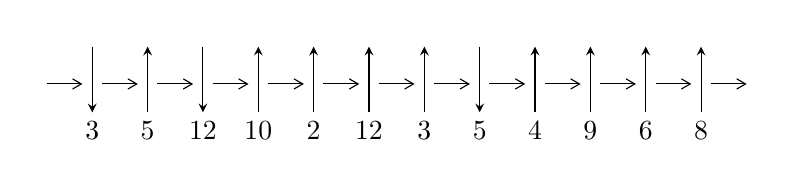
\begin{tikzpicture}[x=20pt, y=17pt]
	% nodes
	\node (C0) at (0, 0) {};
	\node (C1) at (1, 0) {};
	\node (C1U) at (1, +1) {};
	\node (C1D) at (1, -1) {3};

	\node (C2) at (2, 0) {};
	\node (C2U) at (2, +1) {};
	\node (C2D) at (2, -1) {5};

	\node (C3) at (3, 0) {};
	\node (C3U) at (3, +1) {};
	\node (C3D) at (3, -1) {12};

	\node (C4) at (4, 0) {};
	\node (C4U) at (4, +1) {};
	\node (C4D) at (4, -1) {10};

	\node (C5) at (5, 0) {};
	\node (C5U) at (5, +1) {};
	\node (C5D) at (5, -1) {2};

	\node (C6) at (6, 0) {};
	\node (C6U) at (6, +1) {};
	\node (C6D) at (6, -1) {12};

	\node (C7) at (7, 0) {};
	\node (C7U) at (7, +1) {};
	\node (C7D) at (7, -1) {3};

	\node (C8) at (8, 0) {};
	\node (C8U) at (8, +1) {};
	\node (C8D) at (8, -1) {5};

	\node (C9) at (9, 0) {};
	\node (C9U) at (9, +1) {};
	\node (C9D) at (9, -1) {4};

	\node (C10) at (10, 0) {};
	\node (C10U) at (10, +1) {};
	\node (C10D) at (10, -1) {9};

	\node (C11) at (11, 0) {};
	\node (C11U) at (11, +1) {};
	\node (C11D) at (11, -1) {6};

	\node (C12) at (12, 0) {};
	\node (C12U) at (12, +1) {};
	\node (C12D) at (12, -1) {8};
	\node (C13) at (13, 0) {};

	% arrows
	\draw[->,>={angle 60}]
	(C0) edge (C1) (C1) edge (C2) (C2) edge (C3) (C3) edge (C4) (C4) edge (C5) (C5) edge (C6) (C6) edge (C7) (C7) edge (C8) (C8) edge (C9) (C9) edge (C10) (C10) edge (C11) (C11) edge (C12) (C12) edge (C13) ;	\draw[->,>=stealth]
	(C1U) edge (C1D) (C2D) edge (C2U) (C3U) edge (C3D) (C4D) edge (C4U) (C5D) edge (C5U) (C6D) edge (C6U) (C7D) edge (C7U) (C8U) edge (C8D) (C9D) edge (C9U) (C10D) edge (C10U) (C11D) edge (C11U) (C12D) edge (C12U) ;
	\end{tikzpicture} \\
\hhline{~~} \\& 
\textbf{Solving Sequence} \\ \cline{2-2} 
 &
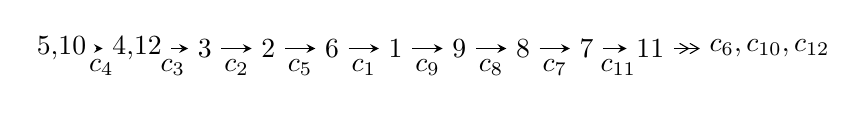
\begin{tikzpicture}[x=23pt, y=7pt]
	% node
	\node (A0) at (-1/8, 0) {5,10};
	\node (A1) at (17/16, 0) {4,12};
	\node (A2) at (17/8, 0) {3};
	\node (A3) at (25/8, 0) {2};
	\node (A4) at (33/8, 0) {6};
	\node (A5) at (41/8, 0) {1};
	\node (A6) at (49/8, 0) {9};
	\node (A7) at (57/8, 0) {8};
	\node (A8) at (65/8, 0) {7};
	\node (A9) at (73/8, 0) {11};
	\node (C1) at (1/2, -1) {$c_{4}$};
	\node (C2) at (13/8, -1) {$c_{3}$};
	\node (C3) at (21/8, -1) {$c_{2}$};
	\node (C4) at (29/8, -1) {$c_{5}$};
	\node (C5) at (37/8, -1) {$c_{1}$};
	\node (C6) at (45/8, -1) {$c_{9}$};
	\node (C7) at (53/8, -1) {$c_{8}$};
	\node (C8) at (61/8, -1) {$c_{7}$};
	\node (C9) at (69/8, -1) {$c_{11}$};
	\node (A10) at (11, 0) {$c_{6},c_{10},c_{12}$};

	% edge
	\draw[->,>=stealth]	
	(A0) edge (A1) (A1) edge (A2) (A2) edge (A3) (A3) edge (A4) (A4) edge (A5) (A5) edge (A6) (A6) edge (A7) (A7) edge (A8) (A8) edge (A9) ;
	\draw[->>,>={angle 60}]	
	(A9) edge (A10);
\end{tikzpicture} \\ 

\end{tabular} \\

\footnotetext{
The image of knot diagram is generated by the software ``\textbf{Draw programme}" developed by Andrew Bartholomew(\url{http://www.layer8.co.uk/maths/draw/index.htm\#Running-draw}), where we modified some parts for our purpose(\url{https://github.com/CATsTAILs/LinksPainter}).
}\phantom \\ \newline 
\centering \textbf{Ideals for irreducible components\footnotemark of $X_{\text{par}}$} 
 
\begin{align*}
I^u_{1}&=\langle 
2.97014\times10^{17} u^{25}-5.76869\times10^{17} u^{24}+\cdots+3.13067\times10^{19} b-2.63141\times10^{17},\\
\phantom{I^u_{1}}&\phantom{= \langle  }1.19380\times10^{20} u^{25}-2.53498\times10^{19} u^{24}+\cdots+5.94827\times10^{20} a-2.01222\times10^{21},\;u^{26}+u^{25}+\cdots-28 u-19\rangle \\
I^u_{2}&=\langle 
- u^{15}+4 u^{13}- u^{12}-10 u^{11}+3 u^{10}+16 u^9-7 u^8-19 u^7+10 u^6+13 u^5-10 u^4-5 u^3+5 u^2+b-1,\\
\phantom{I^u_{2}}&\phantom{= \langle  }-2 u^{15}+u^{14}+6 u^{13}-4 u^{12}-13 u^{11}+9 u^{10}+16 u^9-15 u^8-14 u^7+17 u^6+2 u^5-11 u^4+3 u^3+3 u^2+a-2 u,\\
\phantom{I^u_{2}}&\phantom{= \langle  }u^{16}-4 u^{14}+10 u^{12}-16 u^{10}+u^9+19 u^8-3 u^7-15 u^6+4 u^5+8 u^4-3 u^3-3 u^2+u+1\rangle \\
\\
\end{align*}
\raggedright * 2 irreducible components of $\dim_{\mathbb{C}}=0$, with total 42 representations.\\
\footnotetext{All coefficients of polynomials are rational numbers. But the coefficients are sometimes approximated in decimal forms when there is not enough margin.}
\newpage
\renewcommand{\arraystretch}{1}
\centering \section*{I. $I^u_{1}= \langle 2.97\times10^{17} u^{25}-5.77\times10^{17} u^{24}+\cdots+3.13\times10^{19} b-2.63\times10^{17},\;1.19\times10^{20} u^{25}-2.53\times10^{19} u^{24}+\cdots+5.95\times10^{20} a-2.01\times10^{21},\;u^{26}+u^{25}+\cdots-28 u-19 \rangle$}
\flushleft \textbf{(i) Arc colorings}\\
\begin{tabular}{m{7pt} m{180pt} m{7pt} m{180pt} }
\flushright $a_{5}=$&$\begin{pmatrix}1\\0\end{pmatrix}$ \\
\flushright $a_{10}=$&$\begin{pmatrix}0\\u\end{pmatrix}$ \\
\flushright $a_{4}=$&$\begin{pmatrix}1\\u^2\end{pmatrix}$ \\
\flushright $a_{12}=$&$\begin{pmatrix}-0.200697 u^{25}+0.0426171 u^{24}+\cdots+2.66846 u+3.38286\\-0.00948723 u^{25}+0.0184264 u^{24}+\cdots+0.751262 u+0.00840526\end{pmatrix}$ \\
\flushright $a_{3}=$&$\begin{pmatrix}-0.384928 u^{25}+0.0732483 u^{24}+\cdots+4.20798 u+6.50815\\-0.102054 u^{25}+0.0407047 u^{24}+\cdots+1.29638 u+1.21236\end{pmatrix}$ \\
\flushright $a_{2}=$&$\begin{pmatrix}-0.282874 u^{25}+0.0325436 u^{24}+\cdots+2.91160 u+5.29579\\-0.102054 u^{25}+0.0407047 u^{24}+\cdots+1.29638 u+1.21236\end{pmatrix}$ \\
\flushright $a_{6}=$&$\begin{pmatrix}-0.00386158 u^{25}-0.0616679 u^{24}+\cdots+0.342331 u+1.96390\\0.0590853 u^{25}-0.0329754 u^{24}+\cdots-1.46399 u-0.594028\end{pmatrix}$ \\
\flushright $a_{1}=$&$\begin{pmatrix}-0.326961 u^{25}+0.111690 u^{24}+\cdots+4.32043 u+4.70360\\-0.120257 u^{25}+0.0334802 u^{24}+\cdots+1.90402 u+1.63890\end{pmatrix}$ \\
\flushright $a_{9}=$&$\begin{pmatrix}- u\\- u^3+u\end{pmatrix}$ \\
\flushright $a_{8}=$&$\begin{pmatrix}- u^3\\- u^3+u\end{pmatrix}$ \\
\flushright $a_{7}=$&$\begin{pmatrix}0.0487672 u^{25}+0.135155 u^{24}+\cdots+0.267367 u-3.78355\\-0.000670823 u^{25}+0.0342194 u^{24}+\cdots+0.985487 u-1.00612\end{pmatrix}$ \\
\flushright $a_{11}=$&$\begin{pmatrix}u^3\\u^5- u^3+u\end{pmatrix}$\\&\end{tabular}
\flushleft \textbf{(ii) Obstruction class $= -1$}\\~\\
\flushleft \textbf{(iii) Cusp Shapes $= -\frac{41971186605596834432}{31306709017582656563} u^{25}-\frac{5084666455514062662}{31306709017582656563} u^{24}+\cdots+\frac{725337053465471662059}{31306709017582656563} u+\frac{1192252859670655966978}{31306709017582656563}$}\\~\\
\newpage\renewcommand{\arraystretch}{1}
\flushleft \textbf{(iv) u-Polynomials at the component}\newline \\
\begin{tabular}{m{50pt}|m{274pt}}
Crossings & \hspace{64pt}u-Polynomials at each crossing \\
\hline $$\begin{aligned}c_{1}\end{aligned}$$&$\begin{aligned}
&u^{26}+4 u^{25}+\cdots-5008 u+841
\end{aligned}$\\
\hline $$\begin{aligned}c_{2},c_{5}\end{aligned}$$&$\begin{aligned}
&u^{26}+2 u^{25}+\cdots-152 u+29
\end{aligned}$\\
\hline $$\begin{aligned}c_{3}\end{aligned}$$&$\begin{aligned}
&u^{26}-3 u^{25}+\cdots-4 u+1
\end{aligned}$\\
\hline $$\begin{aligned}c_{4},c_{9}\end{aligned}$$&$\begin{aligned}
&u^{26}+u^{25}+\cdots-28 u-19
\end{aligned}$\\
\hline $$\begin{aligned}c_{6},c_{11}\end{aligned}$$&$\begin{aligned}
&u^{26}+3 u^{25}+\cdots+240 u-56
\end{aligned}$\\
\hline $$\begin{aligned}c_{7}\end{aligned}$$&$\begin{aligned}
&u^{26}+u^{25}+\cdots-9 u+1
\end{aligned}$\\
\hline $$\begin{aligned}c_{8}\end{aligned}$$&$\begin{aligned}
&u^{26}+3 u^{25}+\cdots+1729 u+2888
\end{aligned}$\\
\hline $$\begin{aligned}c_{10}\end{aligned}$$&$\begin{aligned}
&u^{26}-19 u^{25}+\cdots-2570 u+361
\end{aligned}$\\
\hline $$\begin{aligned}c_{12}\end{aligned}$$&$\begin{aligned}
&u^{26}- u^{25}+\cdots+305 u-278
\end{aligned}$\\
\hline
\end{tabular}\\~\\
\newpage\renewcommand{\arraystretch}{1}
\flushleft \textbf{(v) Riley Polynomials at the component}\newline \\
\begin{tabular}{m{50pt}|m{274pt}}
Crossings & \hspace{64pt}Riley Polynomials at each crossing \\
\hline $$\begin{aligned}c_{1}\end{aligned}$$&$\begin{aligned}
&y^{26}+52 y^{25}+\cdots-89120532 y+707281
\end{aligned}$\\
\hline $$\begin{aligned}c_{2},c_{5}\end{aligned}$$&$\begin{aligned}
&y^{26}+4 y^{25}+\cdots-5008 y+841
\end{aligned}$\\
\hline $$\begin{aligned}c_{3}\end{aligned}$$&$\begin{aligned}
&y^{26}+21 y^{25}+\cdots+86 y+1
\end{aligned}$\\
\hline $$\begin{aligned}c_{4},c_{9}\end{aligned}$$&$\begin{aligned}
&y^{26}-19 y^{25}+\cdots-2570 y+361
\end{aligned}$\\
\hline $$\begin{aligned}c_{6},c_{11}\end{aligned}$$&$\begin{aligned}
&y^{26}-33 y^{25}+\cdots+3552 y+3136
\end{aligned}$\\
\hline $$\begin{aligned}c_{7}\end{aligned}$$&$\begin{aligned}
&y^{26}+59 y^{25}+\cdots-63 y+1
\end{aligned}$\\
\hline $$\begin{aligned}c_{8}\end{aligned}$$&$\begin{aligned}
&y^{26}+49 y^{25}+\cdots-13634609 y+8340544
\end{aligned}$\\
\hline $$\begin{aligned}c_{10}\end{aligned}$$&$\begin{aligned}
&y^{26}-15 y^{25}+\cdots-18094 y+130321
\end{aligned}$\\
\hline $$\begin{aligned}c_{12}\end{aligned}$$&$\begin{aligned}
&y^{26}-35 y^{25}+\cdots-343225 y+77284
\end{aligned}$\\
\hline
\end{tabular}\\~\\
\newpage\flushleft \textbf{(vi) Complex Volumes and Cusp Shapes}
$$\begin{array}{c|c|c}  
\text{Solutions to }I^u_{1}& \I (\text{vol} + \sqrt{-1}CS) & \text{Cusp shape}\\
 \hline 
\begin{aligned}
u &= -1.046430 + 0.230334 I \\
a &= \phantom{-}0.904468 + 0.995486 I \\
b &= -0.297194 + 0.524133 I\end{aligned}
 & -2.11030 - 0.82786 I & \phantom{-}9.83528 - 0.62006 I \\ \hline\begin{aligned}
u &= -1.046430 - 0.230334 I \\
a &= \phantom{-}0.904468 - 0.995486 I \\
b &= -0.297194 - 0.524133 I\end{aligned}
 & -2.11030 + 0.82786 I & \phantom{-}9.83528 + 0.62006 I \\ \hline\begin{aligned}
u &= -0.979713 + 0.526985 I \\
a &= \phantom{-}0.47135 - 1.47204 I \\
b &= \phantom{-}0.26056 - 1.46043 I\end{aligned}
 & -6.29591 - 2.05047 I & \phantom{-}2.31530 + 2.39529 I \\ \hline\begin{aligned}
u &= -0.979713 - 0.526985 I \\
a &= \phantom{-}0.47135 + 1.47204 I \\
b &= \phantom{-}0.26056 + 1.46043 I\end{aligned}
 & -6.29591 + 2.05047 I & \phantom{-}2.31530 - 2.39529 I \\ \hline\begin{aligned}
u &= \phantom{-}1.068060 + 0.381172 I \\
a &= \phantom{-}0.25798 + 1.48795 I \\
b &= -1.25101 + 1.49141 I\end{aligned}
 & \phantom{-}3.21406 + 4.68481 I & \phantom{-}6.78577 - 4.01254 I \\ \hline\begin{aligned}
u &= \phantom{-}1.068060 - 0.381172 I \\
a &= \phantom{-}0.25798 - 1.48795 I \\
b &= -1.25101 - 1.49141 I\end{aligned}
 & \phantom{-}3.21406 - 4.68481 I & \phantom{-}6.78577 + 4.01254 I \\ \hline\begin{aligned}
u &= -0.720226 + 0.420524 I \\
a &= \phantom{-}0.109243 + 0.577294 I \\
b &= -0.211859 - 0.068837 I\end{aligned}
 & -1.01337 - 1.74582 I & \phantom{-}2.64941 + 5.86100 I \\ \hline\begin{aligned}
u &= -0.720226 - 0.420524 I \\
a &= \phantom{-}0.109243 - 0.577294 I \\
b &= -0.211859 + 0.068837 I\end{aligned}
 & -1.01337 + 1.74582 I & \phantom{-}2.64941 - 5.86100 I \\ \hline\begin{aligned}
u &= -1.125590 + 0.414878 I \\
a &= -0.60347 + 2.11030 I \\
b &= \phantom{-}0.78890 + 1.53070 I\end{aligned}
 & \phantom{-}3.15440 - 5.95143 I & \phantom{-}5.27054 + 8.12697 I \\ \hline\begin{aligned}
u &= -1.125590 - 0.414878 I \\
a &= -0.60347 - 2.11030 I \\
b &= \phantom{-}0.78890 - 1.53070 I\end{aligned}
 & \phantom{-}3.15440 + 5.95143 I & \phantom{-}5.27054 - 8.12697 I\\
 \hline 
 \end{array}$$\newpage$$\begin{array}{c|c|c}  
\text{Solutions to }I^u_{1}& \I (\text{vol} + \sqrt{-1}CS) & \text{Cusp shape}\\
 \hline 
\begin{aligned}
u &= \phantom{-}0.576799 + 0.539363 I \\
a &= \phantom{-}1.73236 - 0.76798 I \\
b &= \phantom{-}0.917879 + 0.763236 I\end{aligned}
 & \phantom{-}1.72229 - 1.05497 I & \phantom{-}5.11673 - 2.05662 I \\ \hline\begin{aligned}
u &= \phantom{-}0.576799 - 0.539363 I \\
a &= \phantom{-}1.73236 + 0.76798 I \\
b &= \phantom{-}0.917879 - 0.763236 I\end{aligned}
 & \phantom{-}1.72229 + 1.05497 I & \phantom{-}5.11673 + 2.05662 I \\ \hline\begin{aligned}
u &= \phantom{-}0.937850 + 0.875162 I \\
a &= -0.383439 - 0.046876 I \\
b &= \phantom{-}0.058830 - 0.513138 I\end{aligned}
 & -9.63476 + 3.24540 I & \phantom{-}11.28144 - 4.93616 I \\ \hline\begin{aligned}
u &= \phantom{-}0.937850 - 0.875162 I \\
a &= -0.383439 + 0.046876 I \\
b &= \phantom{-}0.058830 + 0.513138 I\end{aligned}
 & -9.63476 - 3.24540 I & \phantom{-}11.28144 + 4.93616 I \\ \hline\begin{aligned}
u &= -0.126374 + 1.299430 I \\
a &= \phantom{-}0.240279 - 0.296936 I \\
b &= \phantom{-}0.23603 - 1.59331 I\end{aligned}
 & \phantom{-}9.18772 + 5.01541 I & \phantom{-}6.86924 - 2.09286 I \\ \hline\begin{aligned}
u &= -0.126374 - 1.299430 I \\
a &= \phantom{-}0.240279 + 0.296936 I \\
b &= \phantom{-}0.23603 + 1.59331 I\end{aligned}
 & \phantom{-}9.18772 - 5.01541 I & \phantom{-}6.86924 + 2.09286 I \\ \hline\begin{aligned}
u &= -0.260661 + 0.600635 I \\
a &= -0.008179 - 0.294986 I \\
b &= -0.523677 + 1.128050 I\end{aligned}
 & \phantom{-}0.64435 + 2.04528 I & \phantom{-}2.89894 - 3.38693 I \\ \hline\begin{aligned}
u &= -0.260661 - 0.600635 I \\
a &= -0.008179 + 0.294986 I \\
b &= -0.523677 - 1.128050 I\end{aligned}
 & \phantom{-}0.64435 - 2.04528 I & \phantom{-}2.89894 + 3.38693 I \\ \hline\begin{aligned}
u &= \phantom{-}0.619771\phantom{ +0.000000I} \\
a &= \phantom{-}0.580980\phantom{ +0.000000I} \\
b &= \phantom{-}0.438499\phantom{ +0.000000I}\end{aligned}
 & \phantom{-}0.786533\phantom{ +0.000000I} & \phantom{-}13.5010\phantom{ +0.000000I} \\ \hline\begin{aligned}
u &= \phantom{-}1.44898 + 0.19387 I \\
a &= \phantom{-}0.44142 + 1.70204 I \\
b &= -0.04602 + 1.63288 I\end{aligned}
 & \phantom{-}6.07568 + 0.67636 I & \phantom{-}9.59349 - 0.33542 I\\
 \hline 
 \end{array}$$\newpage$$\begin{array}{c|c|c}  
\text{Solutions to }I^u_{1}& \I (\text{vol} + \sqrt{-1}CS) & \text{Cusp shape}\\
 \hline 
\begin{aligned}
u &= \phantom{-}1.44898 - 0.19387 I \\
a &= \phantom{-}0.44142 - 1.70204 I \\
b &= -0.04602 - 1.63288 I\end{aligned}
 & \phantom{-}6.07568 - 0.67636 I & \phantom{-}9.59349 + 0.33542 I \\ \hline\begin{aligned}
u &= -1.51509\phantom{ +0.000000I} \\
a &= -0.841913\phantom{ +0.000000I} \\
b &= \phantom{-}0.310960\phantom{ +0.000000I}\end{aligned}
 & \phantom{-}9.26344\phantom{ +0.000000I} & \phantom{-}9.84080\phantom{ +0.000000I} \\ \hline\begin{aligned}
u &= -1.41163 + 0.67471 I \\
a &= \phantom{-}0.68636 - 1.52049 I \\
b &= -0.44218 - 1.83701 I\end{aligned}
 & \phantom{-}13.2089 - 11.9429 I & \phantom{-}8.01117 + 5.02358 I \\ \hline\begin{aligned}
u &= -1.41163 - 0.67471 I \\
a &= \phantom{-}0.68636 + 1.52049 I \\
b &= -0.44218 + 1.83701 I\end{aligned}
 & \phantom{-}13.2089 + 11.9429 I & \phantom{-}8.01117 - 5.02358 I \\ \hline\begin{aligned}
u &= \phantom{-}1.58660 + 0.55037 I \\
a &= -0.82317 - 1.20478 I \\
b &= \phantom{-}0.13502 - 1.49909 I\end{aligned}
 & \phantom{-}14.6555 + 1.7140 I & \phantom{-}9.20177 - 0.71366 I \\ \hline\begin{aligned}
u &= \phantom{-}1.58660 - 0.55037 I \\
a &= -0.82317 + 1.20478 I \\
b &= \phantom{-}0.13502 + 1.49909 I\end{aligned}
 & \phantom{-}14.6555 - 1.7140 I & \phantom{-}9.20177 + 0.71366 I\\
 \hline 
 \end{array}$$\newpage\newpage\renewcommand{\arraystretch}{1}
\centering \section*{II. $I^u_{2}= \langle - u^{15}+4 u^{13}+\cdots+b-1,\;-2 u^{15}+u^{14}+\cdots+a-2 u,\;u^{16}-4 u^{14}+\cdots+u+1 \rangle$}
\flushleft \textbf{(i) Arc colorings}\\
\begin{tabular}{m{7pt} m{180pt} m{7pt} m{180pt} }
\flushright $a_{5}=$&$\begin{pmatrix}1\\0\end{pmatrix}$ \\
\flushright $a_{10}=$&$\begin{pmatrix}0\\u\end{pmatrix}$ \\
\flushright $a_{4}=$&$\begin{pmatrix}1\\u^2\end{pmatrix}$ \\
\flushright $a_{12}=$&$\begin{pmatrix}2 u^{15}- u^{14}+\cdots-3 u^2+2 u\\u^{15}-4 u^{13}+\cdots-5 u^2+1\end{pmatrix}$ \\
\flushright $a_{3}=$&$\begin{pmatrix}2 u^{15}-3 u^{14}+\cdots+2 u+4\\- u^{13}+3 u^{11}-7 u^9+9 u^7- u^6-9 u^5+2 u^4+4 u^3-2 u^2- u+1\end{pmatrix}$ \\
\flushright $a_{2}=$&$\begin{pmatrix}2 u^{15}-3 u^{14}+\cdots+3 u+3\\- u^{13}+3 u^{11}-7 u^9+9 u^7- u^6-9 u^5+2 u^4+4 u^3-2 u^2- u+1\end{pmatrix}$ \\
\flushright $a_{6}=$&$\begin{pmatrix}- u^{15}+4 u^{13}-9 u^{11}+13 u^9- u^8-12 u^7+3 u^6+6 u^5-3 u^4+u^3+u^2+1\\- u^{15}+4 u^{13}+\cdots+3 u^2+2 u\end{pmatrix}$ \\
\flushright $a_{1}=$&$\begin{pmatrix}3 u^{15}- u^{14}+\cdots-4 u^2+u\\u^{15}-4 u^{13}+\cdots- u+1\end{pmatrix}$ \\
\flushright $a_{9}=$&$\begin{pmatrix}- u\\- u^3+u\end{pmatrix}$ \\
\flushright $a_{8}=$&$\begin{pmatrix}- u^3\\- u^3+u\end{pmatrix}$ \\
\flushright $a_{7}=$&$\begin{pmatrix}- u^{15}- u^{14}+\cdots+2 u^2+4 u\\- u^{14}+4 u^{12}+\cdots+3 u+2\end{pmatrix}$ \\
\flushright $a_{11}=$&$\begin{pmatrix}u^3\\u^5- u^3+u\end{pmatrix}$\\&\end{tabular}
\flushleft \textbf{(ii) Obstruction class $= 1$}\\~\\
\flushleft \textbf{(iii) Cusp Shapes $= -8 u^{15}+5 u^{14}+32 u^{13}-19 u^{12}-77 u^{11}+45 u^{10}+119 u^9-78 u^8-125 u^7+100 u^6+79 u^5-84 u^4-20 u^3+38 u^2+2 u-4$}\\~\\
\newpage\renewcommand{\arraystretch}{1}
\flushleft \textbf{(iv) u-Polynomials at the component}\newline \\
\begin{tabular}{m{50pt}|m{274pt}}
Crossings & \hspace{64pt}u-Polynomials at each crossing \\
\hline $$\begin{aligned}c_{1}\end{aligned}$$&$\begin{aligned}
&u^{16}-15 u^{15}+\cdots-19 u+1
\end{aligned}$\\
\hline $$\begin{aligned}c_{2}\end{aligned}$$&$\begin{aligned}
&u^{16}+u^{15}+\cdots+u+1
\end{aligned}$\\
\hline $$\begin{aligned}c_{3}\end{aligned}$$&$\begin{aligned}
&u^{16}+4 u^{15}+\cdots+u+1
\end{aligned}$\\
\hline $$\begin{aligned}c_{4}\end{aligned}$$&$\begin{aligned}
&u^{16}-4 u^{14}+\cdots+u+1
\end{aligned}$\\
\hline $$\begin{aligned}c_{5}\end{aligned}$$&$\begin{aligned}
&u^{16}- u^{15}+\cdots- u+1
\end{aligned}$\\
\hline $$\begin{aligned}c_{6}\end{aligned}$$&$\begin{aligned}
&u^{16}+2 u^{15}+\cdots+2 u^2+1
\end{aligned}$\\
\hline $$\begin{aligned}c_{7}\end{aligned}$$&$\begin{aligned}
&u^{16}+15 u^{14}+\cdots-8 u+1
\end{aligned}$\\
\hline $$\begin{aligned}c_{8}\end{aligned}$$&$\begin{aligned}
&u^{16}-4 u^{14}+\cdots- u+1
\end{aligned}$\\
\hline $$\begin{aligned}c_{9}\end{aligned}$$&$\begin{aligned}
&u^{16}-4 u^{14}+\cdots- u+1
\end{aligned}$\\
\hline $$\begin{aligned}c_{10}\end{aligned}$$&$\begin{aligned}
&u^{16}-8 u^{15}+\cdots-7 u+1
\end{aligned}$\\
\hline $$\begin{aligned}c_{11}\end{aligned}$$&$\begin{aligned}
&u^{16}-2 u^{15}+\cdots+2 u^2+1
\end{aligned}$\\
\hline $$\begin{aligned}c_{12}\end{aligned}$$&$\begin{aligned}
&u^{16}+2 u^{14}+\cdots-2 u+1
\end{aligned}$\\
\hline
\end{tabular}\\~\\
\newpage\renewcommand{\arraystretch}{1}
\flushleft \textbf{(v) Riley Polynomials at the component}\newline \\
\begin{tabular}{m{50pt}|m{274pt}}
Crossings & \hspace{64pt}Riley Polynomials at each crossing \\
\hline $$\begin{aligned}c_{1}\end{aligned}$$&$\begin{aligned}
&y^{16}-13 y^{15}+\cdots-49 y+1
\end{aligned}$\\
\hline $$\begin{aligned}c_{2},c_{5}\end{aligned}$$&$\begin{aligned}
&y^{16}+15 y^{15}+\cdots+19 y+1
\end{aligned}$\\
\hline $$\begin{aligned}c_{3}\end{aligned}$$&$\begin{aligned}
&y^{16}-8 y^{15}+\cdots+y+1
\end{aligned}$\\
\hline $$\begin{aligned}c_{4},c_{9}\end{aligned}$$&$\begin{aligned}
&y^{16}-8 y^{15}+\cdots-7 y+1
\end{aligned}$\\
\hline $$\begin{aligned}c_{6},c_{11}\end{aligned}$$&$\begin{aligned}
&y^{16}+2 y^{15}+\cdots+4 y+1
\end{aligned}$\\
\hline $$\begin{aligned}c_{7}\end{aligned}$$&$\begin{aligned}
&y^{16}+30 y^{15}+\cdots+24 y+1
\end{aligned}$\\
\hline $$\begin{aligned}c_{8}\end{aligned}$$&$\begin{aligned}
&y^{16}-8 y^{15}+\cdots-3 y+1
\end{aligned}$\\
\hline $$\begin{aligned}c_{10}\end{aligned}$$&$\begin{aligned}
&y^{16}+8 y^{15}+\cdots+13 y+1
\end{aligned}$\\
\hline $$\begin{aligned}c_{12}\end{aligned}$$&$\begin{aligned}
&y^{16}+4 y^{15}+\cdots+2 y+1
\end{aligned}$\\
\hline
\end{tabular}\\~\\
\newpage\flushleft \textbf{(vi) Complex Volumes and Cusp Shapes}
$$\begin{array}{c|c|c}  
\text{Solutions to }I^u_{2}& \I (\text{vol} + \sqrt{-1}CS) & \text{Cusp shape}\\
 \hline 
\begin{aligned}
u &= \phantom{-}0.928459 + 0.210985 I \\
a &= -0.08578 + 1.94449 I \\
b &= \phantom{-}0.44492 + 1.40305 I\end{aligned}
 & -5.69032 + 0.91508 I & \phantom{-}6.42574 + 1.46044 I \\ \hline\begin{aligned}
u &= \phantom{-}0.928459 - 0.210985 I \\
a &= -0.08578 - 1.94449 I \\
b &= \phantom{-}0.44492 - 1.40305 I\end{aligned}
 & -5.69032 - 0.91508 I & \phantom{-}6.42574 - 1.46044 I \\ \hline\begin{aligned}
u &= -0.891284 + 0.284250 I \\
a &= \phantom{-}1.049080 + 0.856325 I \\
b &= -0.424111 - 0.038339 I\end{aligned}
 & -2.75842 - 1.23687 I & -0.93586 + 5.66129 I \\ \hline\begin{aligned}
u &= -0.891284 - 0.284250 I \\
a &= \phantom{-}1.049080 - 0.856325 I \\
b &= -0.424111 + 0.038339 I\end{aligned}
 & -2.75842 + 1.23687 I & -0.93586 - 5.66129 I \\ \hline\begin{aligned}
u &= \phantom{-}0.879726 + 0.695218 I \\
a &= -0.783339 - 1.034040 I \\
b &= -0.251596 - 1.308430 I\end{aligned}
 & -5.37416 + 2.67548 I & \phantom{-}8.13212 - 4.78244 I \\ \hline\begin{aligned}
u &= \phantom{-}0.879726 - 0.695218 I \\
a &= -0.783339 + 1.034040 I \\
b &= -0.251596 + 1.308430 I\end{aligned}
 & -5.37416 - 2.67548 I & \phantom{-}8.13212 + 4.78244 I \\ \hline\begin{aligned}
u &= \phantom{-}0.502884 + 0.656202 I \\
a &= \phantom{-}0.921548 + 0.037821 I \\
b &= -0.330221 + 1.286020 I\end{aligned}
 & \phantom{-}1.24395 + 2.85601 I & \phantom{-}7.24981 - 2.90050 I \\ \hline\begin{aligned}
u &= \phantom{-}0.502884 - 0.656202 I \\
a &= \phantom{-}0.921548 - 0.037821 I \\
b &= -0.330221 - 1.286020 I\end{aligned}
 & \phantom{-}1.24395 - 2.85601 I & \phantom{-}7.24981 + 2.90050 I \\ \hline\begin{aligned}
u &= -1.117360 + 0.442159 I \\
a &= -0.68765 + 2.18024 I \\
b &= \phantom{-}0.95379 + 1.98741 I\end{aligned}
 & \phantom{-}4.14272 - 5.66059 I & \phantom{-}13.1246 + 7.2150 I \\ \hline\begin{aligned}
u &= -1.117360 - 0.442159 I \\
a &= -0.68765 - 2.18024 I \\
b &= \phantom{-}0.95379 - 1.98741 I\end{aligned}
 & \phantom{-}4.14272 + 5.66059 I & \phantom{-}13.1246 - 7.2150 I\\
 \hline 
 \end{array}$$\newpage$$\begin{array}{c|c|c}  
\text{Solutions to }I^u_{2}& \I (\text{vol} + \sqrt{-1}CS) & \text{Cusp shape}\\
 \hline 
\begin{aligned}
u &= -0.928870 + 0.835313 I \\
a &= -0.130318 - 0.323140 I \\
b &= \phantom{-}0.141022 + 0.055042 I\end{aligned}
 & -10.05780 - 3.13031 I & -6.80246 + 0.44703 I \\ \hline\begin{aligned}
u &= -0.928870 - 0.835313 I \\
a &= -0.130318 + 0.323140 I \\
b &= \phantom{-}0.141022 - 0.055042 I\end{aligned}
 & -10.05780 + 3.13031 I & -6.80246 - 0.44703 I \\ \hline\begin{aligned}
u &= \phantom{-}1.144080 + 0.550514 I \\
a &= \phantom{-}1.18903 + 1.05584 I \\
b &= -0.11513 + 1.65347 I\end{aligned}
 & \phantom{-}3.33898 + 2.00138 I & \phantom{-}10.41585 - 0.74839 I \\ \hline\begin{aligned}
u &= \phantom{-}1.144080 - 0.550514 I \\
a &= \phantom{-}1.18903 - 1.05584 I \\
b &= -0.11513 - 1.65347 I\end{aligned}
 & \phantom{-}3.33898 - 2.00138 I & \phantom{-}10.41585 + 0.74839 I \\ \hline\begin{aligned}
u &= -0.517636 + 0.368558 I \\
a &= -1.97258 - 0.55483 I \\
b &= -0.91868 + 1.34697 I\end{aligned}
 & \phantom{-}1.99556 + 2.04137 I & \phantom{-}8.89023 - 4.80901 I \\ \hline\begin{aligned}
u &= -0.517636 - 0.368558 I \\
a &= -1.97258 + 0.55483 I \\
b &= -0.91868 - 1.34697 I\end{aligned}
 & \phantom{-}1.99556 - 2.04137 I & \phantom{-}8.89023 + 4.80901 I\\
 \hline 
 \end{array}$$\newpage
\newpage\renewcommand{\arraystretch}{1}
\centering \section*{ III. u-Polynomials}
\begin{tabular}{m{50pt}|m{274pt}}
Crossings & \hspace{64pt}u-Polynomials at each crossing \\
\hline $$\begin{aligned}c_{1}\end{aligned}$$&$\begin{aligned}
&(u^{16}-15 u^{15}+\cdots-19 u+1)(u^{26}+4 u^{25}+\cdots-5008 u+841)
\end{aligned}$\\
\hline $$\begin{aligned}c_{2}\end{aligned}$$&$\begin{aligned}
&(u^{16}+u^{15}+\cdots+u+1)(u^{26}+2 u^{25}+\cdots-152 u+29)
\end{aligned}$\\
\hline $$\begin{aligned}c_{3}\end{aligned}$$&$\begin{aligned}
&(u^{16}+4 u^{15}+\cdots+u+1)(u^{26}-3 u^{25}+\cdots-4 u+1)
\end{aligned}$\\
\hline $$\begin{aligned}c_{4}\end{aligned}$$&$\begin{aligned}
&(u^{16}-4 u^{14}+\cdots+u+1)(u^{26}+u^{25}+\cdots-28 u-19)
\end{aligned}$\\
\hline $$\begin{aligned}c_{5}\end{aligned}$$&$\begin{aligned}
&(u^{16}- u^{15}+\cdots- u+1)(u^{26}+2 u^{25}+\cdots-152 u+29)
\end{aligned}$\\
\hline $$\begin{aligned}c_{6}\end{aligned}$$&$\begin{aligned}
&(u^{16}+2 u^{15}+\cdots+2 u^2+1)(u^{26}+3 u^{25}+\cdots+240 u-56)
\end{aligned}$\\
\hline $$\begin{aligned}c_{7}\end{aligned}$$&$\begin{aligned}
&(u^{16}+15 u^{14}+\cdots-8 u+1)(u^{26}+u^{25}+\cdots-9 u+1)
\end{aligned}$\\
\hline $$\begin{aligned}c_{8}\end{aligned}$$&$\begin{aligned}
&(u^{16}-4 u^{14}+\cdots- u+1)(u^{26}+3 u^{25}+\cdots+1729 u+2888)
\end{aligned}$\\
\hline $$\begin{aligned}c_{9}\end{aligned}$$&$\begin{aligned}
&(u^{16}-4 u^{14}+\cdots- u+1)(u^{26}+u^{25}+\cdots-28 u-19)
\end{aligned}$\\
\hline $$\begin{aligned}c_{10}\end{aligned}$$&$\begin{aligned}
&(u^{16}-8 u^{15}+\cdots-7 u+1)(u^{26}-19 u^{25}+\cdots-2570 u+361)
\end{aligned}$\\
\hline $$\begin{aligned}c_{11}\end{aligned}$$&$\begin{aligned}
&(u^{16}-2 u^{15}+\cdots+2 u^2+1)(u^{26}+3 u^{25}+\cdots+240 u-56)
\end{aligned}$\\
\hline $$\begin{aligned}c_{12}\end{aligned}$$&$\begin{aligned}
&(u^{16}+2 u^{14}+\cdots-2 u+1)(u^{26}- u^{25}+\cdots+305 u-278)
\end{aligned}$\\
\hline
\end{tabular}\newpage\renewcommand{\arraystretch}{1}
\centering \section*{ IV. Riley Polynomials}
\begin{tabular}{m{50pt}|m{274pt}}
Crossings & \hspace{64pt}Riley Polynomials at each crossing \\
\hline $$\begin{aligned}c_{1}\end{aligned}$$&$\begin{aligned}
&(y^{16}-13 y^{15}+\cdots-49 y+1)\\
&\cdot(y^{26}+52 y^{25}+\cdots-89120532 y+707281)
\end{aligned}$\\
\hline $$\begin{aligned}c_{2},c_{5}\end{aligned}$$&$\begin{aligned}
&(y^{16}+15 y^{15}+\cdots+19 y+1)(y^{26}+4 y^{25}+\cdots-5008 y+841)
\end{aligned}$\\
\hline $$\begin{aligned}c_{3}\end{aligned}$$&$\begin{aligned}
&(y^{16}-8 y^{15}+\cdots+y+1)(y^{26}+21 y^{25}+\cdots+86 y+1)
\end{aligned}$\\
\hline $$\begin{aligned}c_{4},c_{9}\end{aligned}$$&$\begin{aligned}
&(y^{16}-8 y^{15}+\cdots-7 y+1)(y^{26}-19 y^{25}+\cdots-2570 y+361)
\end{aligned}$\\
\hline $$\begin{aligned}c_{6},c_{11}\end{aligned}$$&$\begin{aligned}
&(y^{16}+2 y^{15}+\cdots+4 y+1)(y^{26}-33 y^{25}+\cdots+3552 y+3136)
\end{aligned}$\\
\hline $$\begin{aligned}c_{7}\end{aligned}$$&$\begin{aligned}
&(y^{16}+30 y^{15}+\cdots+24 y+1)(y^{26}+59 y^{25}+\cdots-63 y+1)
\end{aligned}$\\
\hline $$\begin{aligned}c_{8}\end{aligned}$$&$\begin{aligned}
&(y^{16}-8 y^{15}+\cdots-3 y+1)\\
&\cdot(y^{26}+49 y^{25}+\cdots-13634609 y+8340544)
\end{aligned}$\\
\hline $$\begin{aligned}c_{10}\end{aligned}$$&$\begin{aligned}
&(y^{16}+8 y^{15}+\cdots+13 y+1)(y^{26}-15 y^{25}+\cdots-18094 y+130321)
\end{aligned}$\\
\hline $$\begin{aligned}c_{12}\end{aligned}$$&$\begin{aligned}
&(y^{16}+4 y^{15}+\cdots+2 y+1)(y^{26}-35 y^{25}+\cdots-343225 y+77284)
\end{aligned}$\\
\hline
\end{tabular}
\vskip 2pc
\end{document}